\documentclass[twocolumn,10pt]{article}
\usepackage[letterpaper,left=1.95cm,right=1.95cm,top=2.5cm,bottom=3.16cm]{geometry} % Márgenes y demás
\usepackage{natbib}
\usepackage{hyperref}
\input{parametros.sty}  %%Llama el archivo de los estilos

%%%%%%% ENCABEZADO %%%%%%%%%%%%%%%%%%%%

{\title{\fontsize{16}{16}
\vspace*{-0.7cm}
\textbf{
Impacto de la contaminación atmosférica urbana en la ocupación de \textit{Zonotrichia capensis} en Bogotá: Un análisis jerárquico bayesiano
} \\[0.2cm]
\fontsize{12}{12}
\textbf{Impact of Urban Air Pollution on the Occupancy of \textit{Zonotrichia capensis} in Bogotá: A Bayesian Hierarchical Analysis}\\[0.2cm]}
}

\author[1,*]{\fontsize{10pt}{10pt}\selectfont \textbf{Nicolás Cárdenas Díaz}}
\author[2]{\textbf{Miguel Ángel Camargo Mora}}
\author[1,3]{\textbf{Brayan Camilo Hernández Silva}}


\affil[1]{
\fontsize{8pt}{8pt}\selectfont Pregrado Ciencia de Datos Universidad Externado, Bogotá - Colombia}
\fontsize{8}{8}
\affil[2]{Pregrado Ciencia de Datos Universidad Externado, Bogotá - Colombia}
\affil[3]{Pregrado Ciencia de Datos Universidad Externado, Bogotá - Colombia \vspace{0.2cm}} 
\affil[*]{nicolas.cardenas1@est.uexternado.edu.co \\
miguel.camargo2@est.uexternado.edu.co \\
brayan.hernandez3@est.uexternado.edu.co}



%%%%%%%%%%%%%%%%%%%%%%%%%%%%%%%%% INICIO DEL DOCUMENTO
%%%%%%%%%%%%%%%%%%%%%%%%%%%%%%%%%%%%%%%%%%%%%%%%%%%%%%%%%%%%%%%%%%%%%%%


\begin{document}
\twocolumn
[
\begin{@twocolumnfalse}
\maketitle
\begin{abstract}
\vspace*{0.5cm}
\justify
\fontsize{10pt}{10pt}\selectfont

La contaminación atmosférica representa una amenaza creciente para la biodiversidad urbana, pero su efecto sobre la distribución de aves neotropicales ha sido poco estudiado en ciudades latinoamericanas. En este trabajo, analizamos cómo los niveles de material particulado ($\text{PM}_{10}$) y ozono ($\text{O}_3$) se relacionan con la presencia del copetón (\textit{Zonotrichia capensis}) en Bogotá. Para esto, integramos registros de la plataforma de ciencia ciudadana eBird con datos de la Red de Monitoreo de Calidad del Aire de Bogotá (RMCAB). Implementamos un modelo bayesiano de ocupación que nos permite corregir los errores de observación y distinguir entre la ausencia real del ave y el hecho de que simplemente no haya sido vista. Al usar un enfoque probabilístico con distribuciones que se ajustan a los datos, buscamos determinar si la polución reduce significativamente la presencia de esta especie en la capital. Con ello, este trabajo busca responder una pregunta concreta: ¿afecta la contaminación atmosférica urbana la probabilidad de observar al copetón en Bogotá?

\keywordsSpan{Modelo de ocupación, Estadística bayesiana, Pólya-Gamma, Contaminación atmosférica, \textit{Zonotrichia capensis}, eBird, Bogotá}
\end{abstract}
\vspace{0.5cm}



\renewcommand{\abstractname}{ABSTRACT}
\begin{abstract}
\vspace*{0.5cm}
\justify

\textit{Air pollution is a growing threat to urban biodiversity, yet its effect on Neotropical birds remains poorly understood in Latin American cities. In this study, we analyze how particulate matter ($\text{PM}_{10}$) and ozone ($\text{O}_3$) levels affect the occurrence of the Rufous-collared Sparrow (\textit{Zonotrichia capensis}) in Bogotá. We integrated records from the eBird citizen science platform with data from Bogotá's Air Quality Monitoring Network (RMCAB). We implemented a Bayesian occupancy model to separate the actual presence of the bird from observation errors, ensuring that the results account for the uncertainty inherent in citizen science data. By using a data-driven probabilistic approach, we aim to determine if air pollution significantly reduces the presence of this species in the city. This work seeks to answer a concrete question: does urban air pollution affect the probability of observing the Rufous-collared Sparrow in Bogotá?}

\keywordsEng{Occupancy model, Bayesian statistics, Pólya-Gamma, Air pollution, \textit{Zonotrichia capensis}, eBird, Bogotá}
\end{abstract}

\vspace*{0.5cm}  %%% Espacio entre el abstract y las columnas

\end{@twocolumnfalse}
]


\thispagestyle{alim}


\section{INTRODUCCIÓN}

\justifying
Para los habitantes de Bogotá, el amanecer no comienza con el ruido del tráfico, sino con el canto rítmico del copetón (\textit{Zonotrichia capensis}). Esta pequeña ave, que ha logrado adaptarse a la expansión de ladrillo y asfalto de la capital, es más que un habitante urbano; representa la banda sonora de parques, jardines y humedales. Sin embargo, mientras la ciudadanía se habitúa a los niveles de polución que tiñen el cielo, surge la necesidad de cuestionar el impacto sobre aquellas especies que no pueden elegir el aire que respiran. Bogotá es una de las urbes más pobladas y contaminadas de Latinoamérica; se estima que de haber mantenido concentraciones promedio anuales de $PM_{2.5}$ en 5 µg/m³ se habrían evitado aproximadamente 13.345 muertes en personas mayores de 30 años entre 2018 y 2022 \cite{SDS2023}. De igual manera, sustancias como el material particulado grueso ($\text{PM}_{10}$) y el ozono ($\text{O}_3$) superan constantemente los umbrales considerados seguros. Aunque los efectos sobre la salud pública son evidentes, el impacto en la biodiversidad urbana nativa permanece, en gran medida, como una problemática poco explorada de forma cuantitativa.

El copetón se presenta como el sujeto de estudio ideal para evaluar esta realidad ecológica. Al encontrarse distribuido por toda la geografía urbana, ofrece una oportunidad única para responder una interrogante central en la ecología urbana neotropical:

\vspace{0.2cm}
\noindent\textit{¿Cómo afectan los niveles de contaminación atmosférica urbana a la probabilidad de observar al copetón (\textit{Zonotrichia capensis}) en la ciudad de Bogotá?}
\vspace{0.2cm}

Existen antecedentes internacionales que apuntan hacia una respuesta preocupante. En contextos urbanos, \cite{ortega2011} y \cite{silva2022} han demostrado que diversas formas de perturbación ambiental reducen la presencia de aves nativas. Desde la perspectiva biológica, \cite{sanderfoot2017} explicaron que las aves son especialmente vulnerables a los tóxicos atmosféricos debido a que su sistema respiratorio, a diferencia del humano, absorbe gases de forma continua y unidireccional. Además, \cite{dugger2021} descubrieron que la contaminación puede provocar que los observadores dejen de detectar individuos antes de que estos desaparezcan realmente de un sitio, lo cual obliga a separar matemáticamente el proceso de ocupación real del proceso de observación.

Para resolver este desafío estadístico, se recurre a los \textbf{modelos de ocupación}, introducidos por \cite{mackenzie2002}. Estos modelos dividen el análisis en dos capas jerárquicas: una que estima la probabilidad real de que el ave ocupe un sitio (ocupación, $\psi$), y otra que estima la probabilidad de que un observador la registre dado que está presente (detección, $p$). Para ajustar estos modelos bajo un enfoque bayesiano eficiente, \cite{clark2019} propusieron el uso del aumento de datos de Pólya-Gamma \citep{polson2013}, técnica que simplifica los cálculos y permite obtener resultados precisos sin recurrir a aproximaciones computacionalmente costosas.

Con estos elementos, el objetivo de este estudio es determinar si los niveles de $\text{PM}_{10}$ y $\text{O}_3$ están asociados con una menor probabilidad de ocupación del copetón en Bogotá. Para lograrlo, se propusieron los siguientes objetivos específicos: (1) integrar los registros de avistamientos de eBird \citep{sullivan2009} con los datos horarios de la Red de Monitoreo de Calidad del Aire de Bogotá (RMCAB); (2) ajustar un modelo bayesiano jerárquico con distribuciones a priori no informativas; y (3) evaluar los efectos mediante intervalos de credibilidad al 95\%.

\section{Análisis Exploratorio}

\justifying
Esta sección detalla el comportamiento estadístico de la base de datos combinada de avistamientos (eBird, \url{https://ebird.org}) y calidad del aire (RMCAB, \url{http://rmcab.ambientebogota.gov.co}). Al explorar los datos, se busca identificar los desafíos ambientales y metodológicos que el modelo posterior deberá resolver.

\subsection{Análisis Descriptivo}

El dataset consolidado cuenta con \textbf{910 unidades de muestreo}. El análisis inicial de las variables ambientales ($\text{PM}_{10}, \text{PM}_{2.5}, \text{CO}, \text{NO}_2, \text{O}_3, \text{SO}_2$) y de esfuerzo ($\text{duración, distancia, observadores}$) reveló dos características críticas: la completitud incompleta y la falta de simetría.

\textbf{Completitud e Histograma:}
Los contaminantes particulados ($\text{PM}_{10}$ y $\text{PM}_{2.5}$) mostraron una completitud excelente ($\sim$98.5\% de datos presentes). Sin embargo, los contaminantes gaseosos como el $\text{NO}_2$ y el $\text{CO}$ presentaron déficits de información superiores al 40\%, lo cual sugería el riesgo de inducir falsas certezas si se incluían en el modelado. Respecto a la distribución, como se detalla en la sección de gráficas, todas las variables presentan un sesgo positivo marcado, lo que confirma que la polución en Bogotá opera bajo eventos de picos esporádicos sobre una base de niveles bajos estables.

\subsubsection{Procesamiento de Datos}

La preparación de la información se dividió en tres fases técnicas diseñadas para garantizar la rigurosidad del estudio:

\begin{enumerate}
    \item \textbf{Cruce Espaciotemporal:} Mediante algoritmos de distancia geométrica en Python, se vinculó cada avistamiento con la estación de la RMCAB más cercana en el momento exacto de la observación.
    \item \textbf{Filtrado de Calidad (Listas Completas):} Se excluyeron los registros parciales para asegurar el cumplimiento del supuesto de ocupación. El uso de \textbf{Listas Completas} de eBird garantiza que la ausencia de registro del copetón sea interpretada matemáticamente como una probable ausencia real de la especie.
    \item \textbf{Estandarización ($Z$-score):} Se realizó el re-escalado de las variables continuas ($\mu=0, \sigma=1$) para garantizar: (1) la \textbf{convergencia acelerada} del algoritmo Gibbs; (2) la \textbf{comparabilidad directa} entre los efectos de los contaminantes independientemente de sus unidades originales; y (3) la \textbf{alineación logística} con las distribuciones a priori $\mathcal{N}(0,1)$ empleadas.
\end{enumerate}

\subsection{Presentación de Gráficas}

A continuación, se presentan las gráficas pertinentes para comprender la naturaleza de los datos y sustentar la elección de variables del modelo.

\begin{figure}[H]
    \centering
    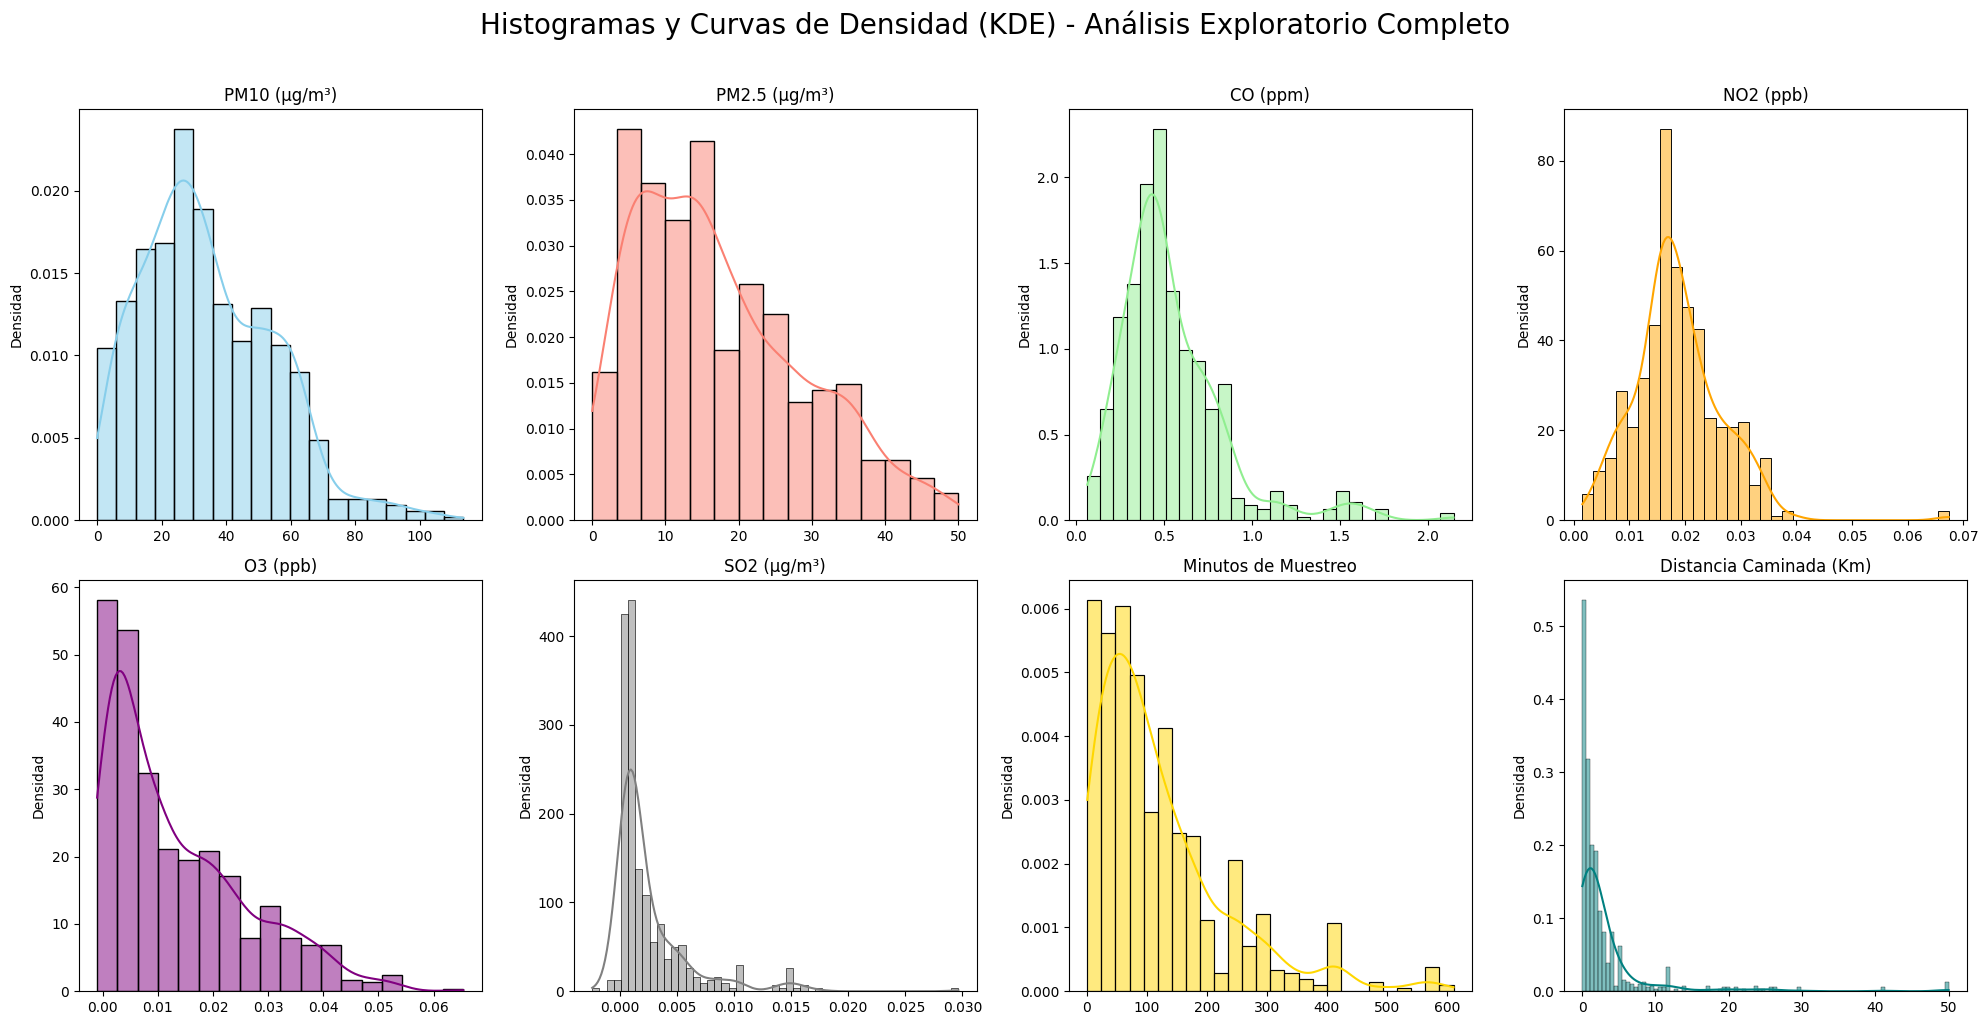
\includegraphics[width=\columnwidth]{Figuras/density_plots_all.png}
    \caption{Curvas de densidad (KDE). Se observa la asimetría positiva en todas las variables ambientales y de esfuerzo.}
    \label{fig:density}
\end{figure}

Al analizar la Figura \ref{fig:density}, se observa que ninguna de las variables sigue una distribución normal simétrica. Todas presentan un marcado sesgo positivo (cola hacia la derecha), lo cual es coherente con la dinámica ambiental de Bogotá: predominan los niveles bajos y estables de polución, interrumpidos por eventos esporádicos de alta contaminación. Este hallazgo descarta el uso de pruebas estadísticas clásicas que asumen normalidad y justifica plenamente el enfoque bayesiano. Las variables numéricas continuas identificadas para este proceso, y que han sido sometidas a estandarización ($Z$-score) para el modelado, son: \texttt{pm10\_ugm3}, \texttt{o3\_ppb} y \texttt{DURATION MINUTES}.

\begin{figure}[H]
    \centering
    
\includegraphics[width=\columnwidth]{Figuras/correlation_matrix.png}
    \caption{Matriz de Correlación de Spearman. Resalta la alta redundancia ($\rho=0.77$) entre el $\text{PM}_{10}$ y $\text{PM}_{2.5}$.}
    \label{fig:corrmatrix}
\end{figure}

La Figura \ref{fig:corrmatrix} revela una independencia deseable entre la mayoría de las variables. No obstante, se detectó una multicolinealidad fuerte entre el $\text{PM}_{10}$ y el $\text{PM}_{2.5}$ ($\rho=0.77$). Para evitar redundancia en el modelo, se seleccionó únicamente el $\text{PM}_{10}$, dado que representa de forma más precisa el material particulado que se deposita en el estrato bajo donde forrajea habitualmente el copetón.

\begin{figure}[H]
    \centering
    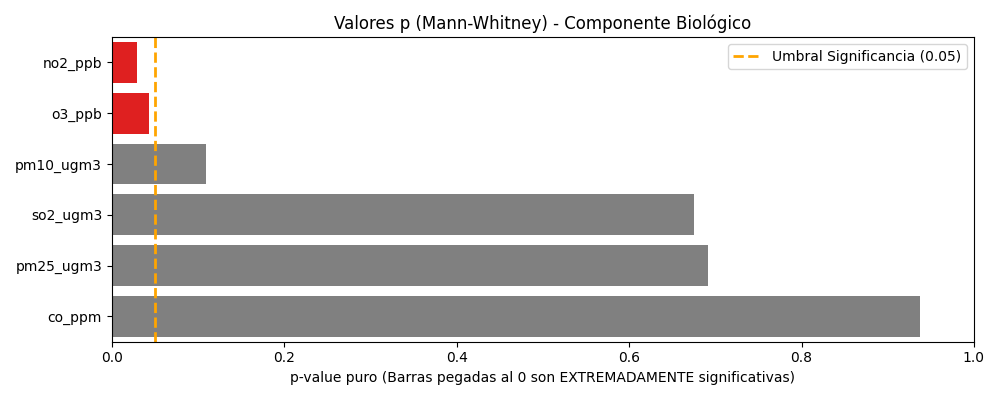
\includegraphics[width=\columnwidth]{Figuras/pvalues_mannwhitney_bio.png}
    \caption{Valores-P de Mann-Whitney para contaminantes. Solo el $O_3$ muestra significancia preliminar univariada.}
    \label{fig:pvalues_bio}
\end{figure}

A nivel univariado, la Figura \ref{fig:pvalues_bio} sugiere que solo el $\text{O}_3$ presenta diferencias significativas ($p < 0.05$) entre sitios con presencia y ausencia del ave. Aunque el $\text{PM}_{10}$ no superó este umbral inicial, se retuvo para el modelo bayesiano jerárquico, ya que este es capaz de detectar efectos ecológicos que las pruebas simples ignoran al no controlar por el esfuerzo de observación.

\begin{figure}[H]
    \centering
    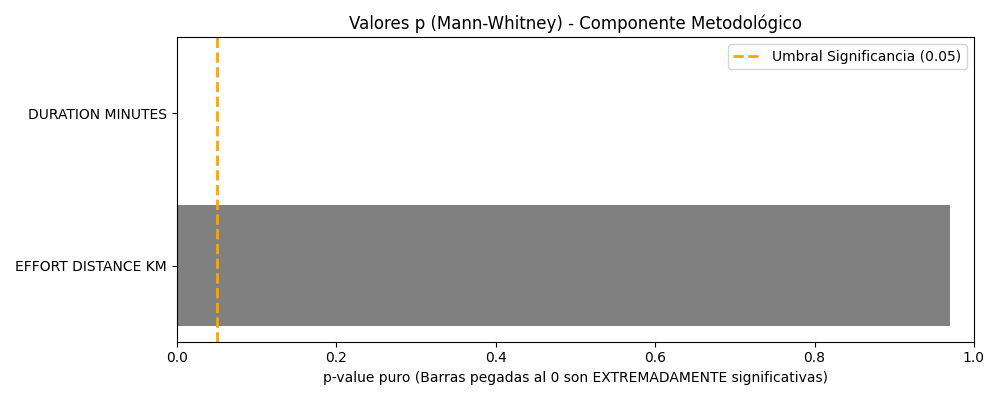
\includegraphics[width=\columnwidth]{Figuras/pvalues_mannwhitney_method.png}
    \caption{Valores-P para esfuerzo humano. La duración de la observación es el factor crítico de detección ($p < 0.0001$).}
    \label{fig:pvalues_method}
\end{figure}

La Figura \ref{fig:pvalues_method} arroja un hallazgo metodológico crucial: la duración de la observación es extremadamente significativa ($p < 0.0001$), mientras que la distancia recorrida es irrelevante ($p = 0.96$). Esto indica que, para observar al copetón, es más determinante la paciencia del observador que el desplazamiento físico realizado en el campo.

\begin{figure}[H]
    \centering
    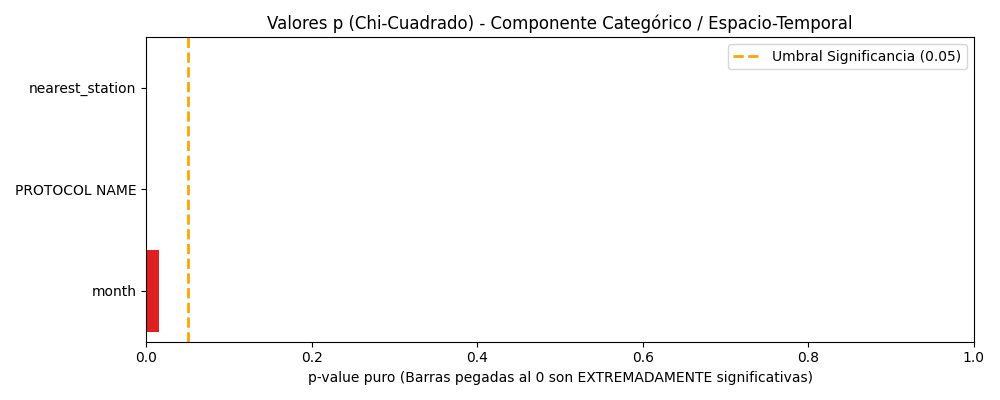
\includegraphics[width=\columnwidth]{Figuras/pvalues_chisquare.png}
    \caption{Pruebas de Chi-Cuadrado para variables geográficas. La estación de monitoreo es un control espacial obligatorio.}
    \label{fig:pvalues_chi2}
\end{figure}

Finalmente, la Figura \ref{fig:pvalues_chi2} confirma que la estación de monitoreo y el protocolo de observación son factores espaciotemporales determinantes ($p < 0.0001$). Esto obliga a considerar la ubicación geográfica como una variable de control fundamental para evitar sesgos derivados de la heterogeneidad del entorno urbano bogotano.

Como síntesis del análisis exploratorio, el modelo se construirá utilizando la siguiente arquitectura de variables: para el componente biológico de ocupación ($\psi$) se seleccionaron el intercepto, \texttt{pm10\_ugm3} y \texttt{o3\_ppb}; para el componente de detección ($p$) se utilizarán el intercepto, \texttt{DURATION MINUTES}, \texttt{PROTOCOL NAME} y \texttt{nearest\_station} como controles obligatorios.

\subsection{Presentación de las Hipótesis}

Basándose en la exploración visual y las pruebas de hipótesis realizadas, se establecen las siguientes hipótesis de trabajo:

\begin{itemize}
    \item \textbf{Hipótesis 1 (Ambiental):} La ocupación del copetón está inversamente relacionada con los niveles de $\text{PM}_{10}$ y $\text{O}_3$, debido al estrés respiratorio que estos contaminantes generan en aves de estrato bajo.
    \item \textbf{Hipótesis 2 (Metodológica):} La probabilidad de detectar al ave depende positivamente del tiempo de observación (duración) y varía significativamente según la ubicación geográfica (control por estación).
    \item \textbf{Hipótesis 3 (Bayesiana):} El uso de un modelo jerárquico permitirá recuperar el efecto real de la contaminación al descontar el ruido generado por la imperfección en la detección humana.
\end{itemize}

\section{Modelo de regresión}

\justifying
Esta sección formaliza la arquitectura matemática del modelo diseñado para procesar los datos consolidados. Se emplea un \textbf{Modelo Jerárquico Bayesiano de Ocupación} que separa el estado ecológico real de la especie (ocupación latente $\psi$) del error de observación (detección $p$), siguiendo la formulación de \cite{clark2019} con aumento de datos de Pólya-Gamma.

\subsection{Separación de Parámetros: Beta vs. Alpha}

En los modelos jerárquicos de ocupación se independiza el ecosistema real del error observacional. El modelo se estructura en dos componentes:

\begin{itemize}
  \item \textbf{Proceso Ecológico (Parámetros Beta, $\beta$):} Modelan la \textbf{biología} de la especie (Ocupación latente $\psi$). Responden a si el entorno permite que el ave resida en el sitio. Cuentan con un intercepto ecológico base ($\beta_0$).
  \item \textbf{Proceso de Observación (Parámetros Alpha, $\alpha$):} Modelan el \textbf{error observacional} (Detección $p$). Responden a si el observador logró registrar al individuo asumiendo que estaba presente. Cuentan con un intercepto de detectabilidad base ($\alpha_0$).
\end{itemize}

\subsection{Especificación y Justificación de las Priors}

Para cada coeficiente de las regresiones, se asignó una distribución previa asumiendo ignorancia inicial pero permitiendo que el muestreo converja. Para garantizar la integridad científica del estudio, todas las pre-creencias sobre los coeficientes se modelan con \textbf{Distribuciones Normales no informativas} independientes:

\begin{align}
  \beta_0,\, \beta_{\text{pm10\_ugm3}},\, \beta_{\text{o3\_ppb}} &\sim \mathcal{N}(0,\, 1) \\
  \alpha_0,\, \alpha_{\text{DURATION MINUTES}},\, \alpha_{\text{nearest\_station}},\, \alpha_{\text{PROTOCOL NAME}} &\sim \mathcal{N}(0,\, 1)
\end{align}

Adicionalmente, se define la prior para la variable latente del aumento de datos:
\begin{equation}
    \omega \sim \mathcal{PG}(b=1,\, c=0)
\end{equation}

Donde la distribución Pólya-Gamma se ancla en $b=1$ al estar condicionada a la verosimilitud binaria y se fija $c=0$ para mantener una media neutra. El uso de la prioridad $\mathcal{N}(0, 1)$ se fundamenta en una \textbf{premisa de objetividad por falta de experticia a priori}. Dado que no se cuenta con conocimiento ornitológico previo que permita asegurar puntualmente el nivel de toxicidad del ozono sobre los pulmones de \textit{Z. capensis}, se asume una expectativa central neutra ($\mu_0 = 0$).

\subsection{La Likelihood y el Acomodamiento Pólya-Gamma}

El proceso sigue una jerarquía de tres etapas diseñada para transformar un problema binario difícil en una estructura lineal tratable, vinculando la biología real con la observación humana:

\textbf{1. La Naturaleza Jerárquica (Unión de Bernoullis):} El modelo se construye sobre dos capas estocásticas encadenadas. Primero, el estado real de ocupación del ave en el sitio $i$ ($z_i$):
\begin{equation}
   z_i \sim \text{Bernoulli}(\psi_i)
\end{equation}

Segundo, el éxito de detección en la visita $j$ del sitio $i$ ($y_{i,j}$), el cual está estrictamente condicionado a la presencia real ($z_i$):
\begin{equation}
   y_{i,j} \sim \text{Bernoulli}(z_i \cdot p_{i,j})
\end{equation}

Esta estructura demuestra que si el ave no ocupa el sitio ($z_i=0$), la probabilidad de detección es nula ($0 \cdot p = 0$). La \textbf{Verosimilitud Conjunta} (Likelihood) para los $N$ sitios y $K_i$ visitas se define como el producto de ambas capas:
\begin{equation}
  L\!\left(y, z \mid \beta, \alpha\right) = \prod_{i=1}^N \left[ \text{Bernoulli}(z_i \mid \psi_i) \prod_{j=1}^{K_i} \text{Bernoulli}(y_{i,j} \mid z_i \cdot p_{i,j}) \right]
  \label{eq:likelihood_joint}
\end{equation}

\textbf{2. El Enlace Logístico (Inverse-Logit):} Para establecer el vínculo con las covariables ambientales ($\beta$) y de esfuerzo ($\alpha$), se aplica la función logística:
\begin{equation}
  \psi_i = \frac{e^{X_i\beta}}{1 + e^{X_i\beta}}, \quad p_{i,j} = \frac{e^{W_{i,j}\alpha}}{1 + e^{W_{i,j}\alpha}}
\end{equation}

\textbf{3. Acondicionamiento Estocástico (Identidad PG):} Debido a que el denominador logístico es no lineal, se aplica la identidad de \cite{polson2013}. Esta permite reescribir la verosimilitud como una integral de una distribución Normal ponderada por la variable latente $\omega \sim \mathcal{PG}(1, 0)$:

\begin{equation}
  \underbrace{\dfrac{(e^\psi)^y}{1+e^\psi}}_{\text{Logit}} = \text{Capa Lineal} \cdot \int_0^\infty \underbrace{\exp \left( -\frac{\omega \psi^2}{2} \right)}_{\text{Capa Cuadrática (Normal)}} p(\omega \mid 1, 0) d\omega
\end{equation}

La variable \textbf{Pólya-Gamma ($\omega$)} actúa como un transformador que genera un peso para "enderezar" localmente la curva logística. Al convertir el problema binario en una estructura cuadrática (Normal), se logra una solución cerrada que permite determinar si los coeficientes de contaminación (\texttt{pm10\_ugm3}, \texttt{o3\_ppb}) tienen un efecto significativamente negativo una vez descontado el ruido de detección.


\section{CONCLUSIÓN}

\justifying
\textit{Sección por desarrollar tras el análisis de los resultados.}


\bibliographystyle{apalike}
\bibliography{Bibliografia}

\end{document}








































































































\end{document}
